\section{Project management, consideration of sustainability and health and safety}

\label{sec:conclusion}
\subsection{Project management}

The primary tool for managing the project was a Gantt chart, as illustrated in \autoref{fig:gantt_chart}. This chart served as a visual tool to set and track realistic timelines for completing various sections of the project. It was updated throughout the project to reflect changes, including additions and deletions of project segments.

Regular updates to the chart, combined with weekly meetings with the supervisor, ensured the project remained on schedule.

% 管理项目的主要工具是甘特图,如图所示。这个图表作为一个可视化工具,用于设定和跟踪完成项目各个部分的实际时间表。在整个项目过程中,它会不断更新,以反映项目段落的增加和删除。

% 通过定期更新图表,并结合每周与导师的会议,确保了项目按计划进行。

\begin{figure}[htbp]
    \centering
    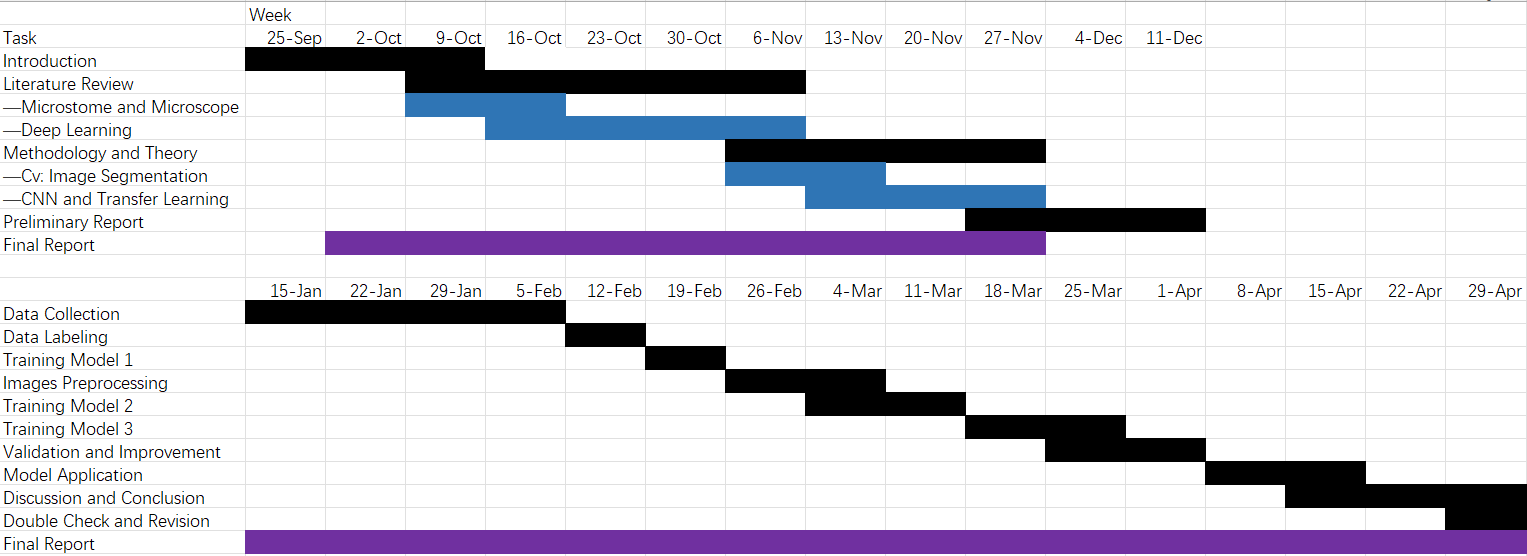
\includegraphics[width=1\textwidth]{./fig/gantt_chart.png}
    \caption{Gantt chart}
    \label{fig:gantt_chart}
\end{figure}


% \subsection{Health and safety}

% 在实验中唯一能产生安全风险的就是实验仪器的操作,其中主要风险是在制备生物切片和显微镜的操作。在制备切片是将会使用非常锋利的组织切片刀,因此在操作时需要特别小心,以免切到手指。我们在操作时严格遵守实验规范,戴上手套,避免直接接触刀片。此外,为了避免误伤和保证实验的一致性,在大部分情况下我们都使用机器的自动切削功能,而不是手动切削。这也就是说,在制备切片的过程中,实验人员仅仅负责对刀而剩下的事情都是由机器来完成的。

% 在显微镜采集图像时,主要风险是在调节显微镜时,不小心碰到显微镜的镜片,导致镜片破损。为了避免这种情况的发生,我们在操作时都尽量避免手工操作,而是通过显微镜的自动调节功能来调节焦距和光圈大小。这样能够避免在触摸转动显微镜头的同时污染镜头,导致成像质量的下降。

% \subsection{Sustainability}

% 有关于可持续性的考虑,在实验中的产物只有生物组织切片和玻璃片。对于这些已经使用的物品,我们严格按照垃圾分类的要求进行处理。对于生物组织切片,我们将其刮下并放入生物垃圾桶中,而对于玻璃片,特别考虑到其的锋利程度,我们需要将其进行简单包装后放入玻璃垃圾桶中。这样能够保证实验室的环境整洁,也能够保护实验人员的安全,避免被锋利尖锐物品误伤。

% 此外,关于实验室用电和能源节约的相关事项,我们还是采用了一些简单的常识性节能措施。在离开时确保机器已经完全关闭,用以减少能源的浪费。这些措施虽然看似微不足道,但是在长期的实验过程中,能够为环境保护和节约能源做出一定的贡献。

\subsection{Health and Safety}

The only potential safety hazards in the laboratory stem from the operation of experimental equipment, particularly during the preparation of biological sections and the use of microscopes. The preparation of sections involves the use of extremely sharp tissue slicers, necessitating great caution to avoid cutting fingers. We adhere strictly to laboratory protocols, wearing gloves and avoiding direct contact with blades. Moreover, to minimize injuries and ensure consistency in experiments, we mostly employ the automatic cutting function of the machine rather than manual cutting. This means that during the section preparation process, the experimenter is only responsible for adjusting the blade while the machine handles the rest.

While capturing images under the microscope, the primary risk involves accidentally touching the microscope's lenses, which could damage them. To prevent this, we minimize manual handling and utilize the microscope's automatic adjustment features to control focus and aperture. This approach helps prevent contamination of the lens during manual adjustments, thereby maintaining the quality of imaging.

\subsection{Sustainability}

Concerning sustainability, the only outputs from our experiments are biological tissue sections and glass slides. These used materials are disposed of strictly according to waste segregation protocols. Biological tissue sections are scraped off and placed in biological waste bins, whereas glass slides, given their sharpness, are wrapped and placed in bins designated for glass. These practices ensure a clean laboratory environment and protect personnel from injuries caused by sharp objects.

Additionally, we implement basic energy-saving measures related to the use of electricity and other resources in the lab. Ensuring that equipment is completely turned off when not in use helps to minimize energy wastage. Although these measures may seem minor, they contribute significantly to environmental protection and energy conservation over the long term.









